% outline overall design with figure from pres
% intro subsections

\begin{figure}
    \centering
    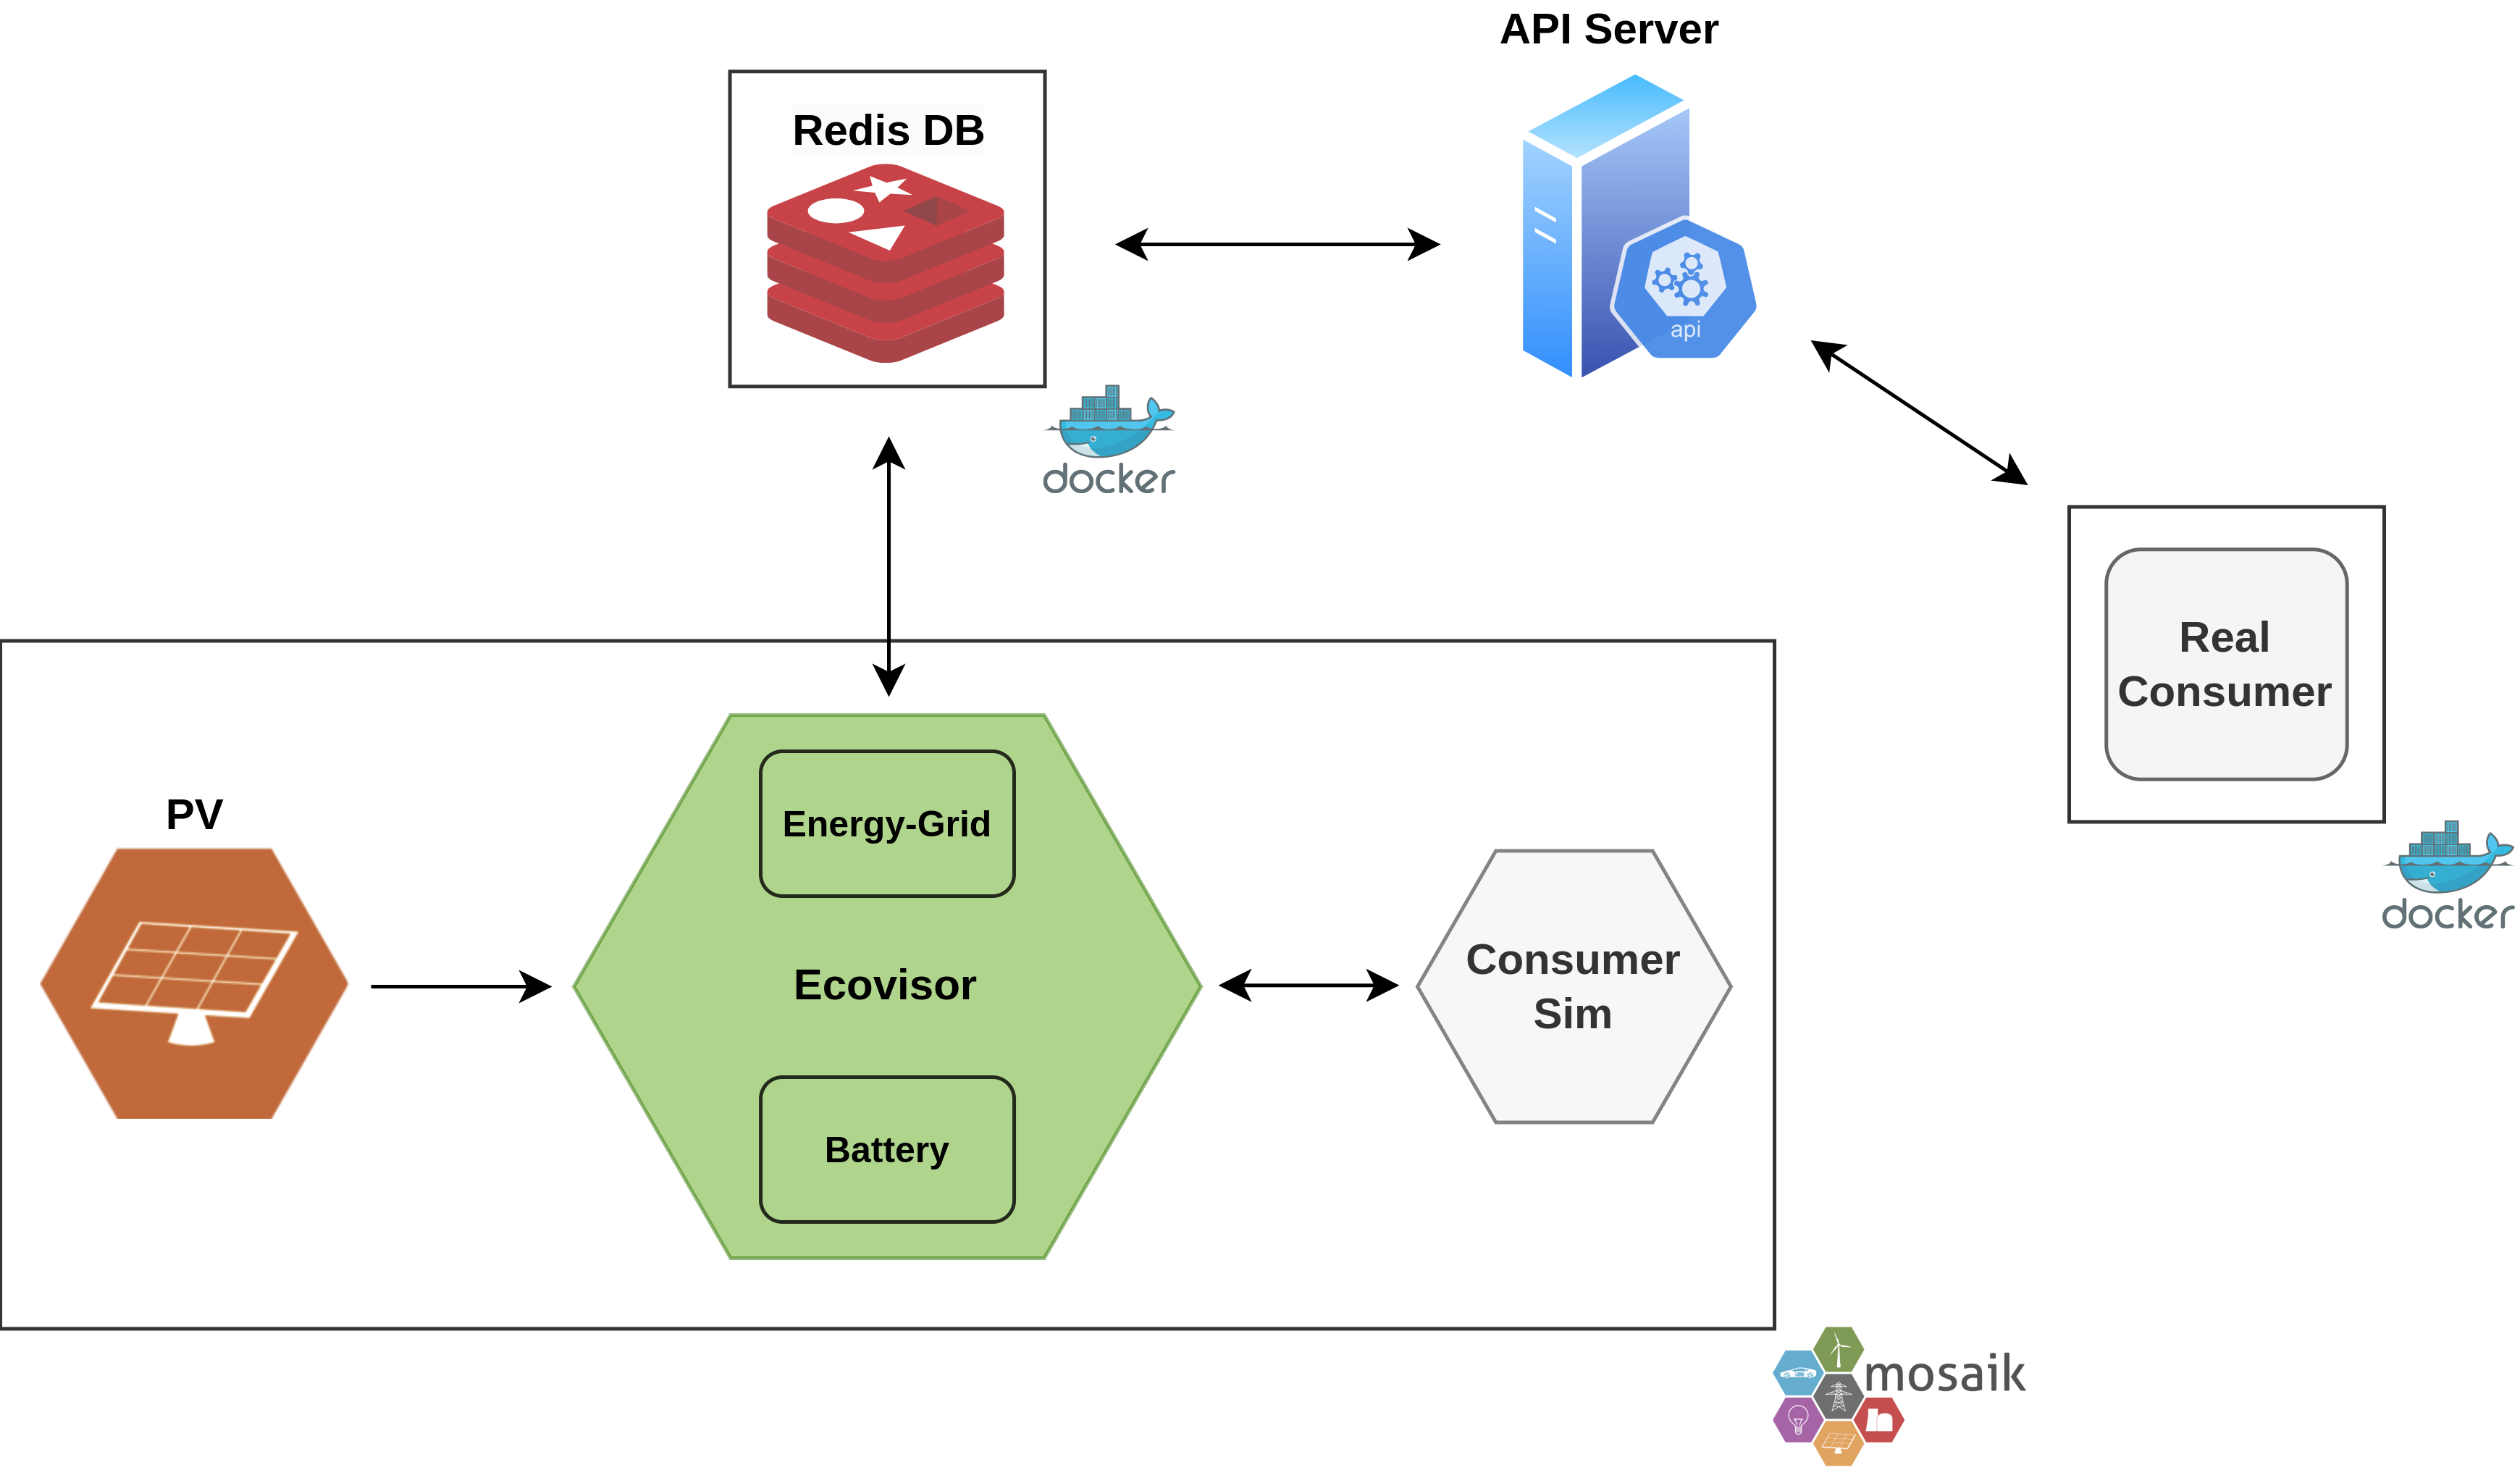
\includegraphics[width=\linewidth]{figures/system_design}
    \caption{System Design}
    \label{fig:system_design}
\end{figure}

\subsection{Simulation of the Ecovisor}

\subsection{Interface to External Applications}
ToDo: Second itteration on writing

For connecting the Ecovisor-Model to a real workload, we had to expose the API described in \cite{souza2023}. We have tried to implement it as it would probably be implemented in a real cloud environment. %source?
To achive that, we implemented the API of the Ecoviser with a RedisDB as value store between the ecovisor and the api-server. This also ensures atomiticity on the writes of the values. %sourec

%Picture API

%Picture Data-Flow (Values set by Ecovisor, Values set by Workload)

\subsubsection{API-Server}
The API Server exposes the Ecoviser-APi to the "Workloads". It is implemented with the FastAPI Framework and Utilizes Uviorn to handel multiple clients accessing the API.
The Module is started as aan independent thread. In earlyer versions we tried to implement it inside of the ecovisor model, but due to the way uvicorn starts the API-Server,
it would stops the execution of the simulation until the API-Server is stopped and so we decided to design it as a standalone module. This als enables the API-Server to be scaled indipendetn from
the Ecovisor-Model and the RedisDB. This may be helpful in bigger simulations with distributed infrastructur. 


\subsubsection{RedisDB}
The RedisDB is used to interchange the values provided by eiterh ecovisor or the workload application. The database itself is a fast in memory key value store, wich is started as a docker container via the docker python libary %quelle pyton lib
to keep manual managment of the simulation to a minimum. 

In general the Database can be exchanged with any other database by adapting the interface in the ecovisor model. This can be useful when simulation should be integrated 
in a production grade cloud environment like kubernetes or open stack.

%values picture

\subsubsection{Ecovisor-Redis-Interface}
